
\documentclass[12pt]{article}
\usepackage{setspace}
\doublespacing
\usepackage{fullpage}
\usepackage{amsbsy}
\usepackage{amsmath}
\usepackage{amsfonts}
\usepackage{amsthm}
\usepackage{amssymb}
\usepackage{algorithmic}
\usepackage{algorithm}
\usepackage{enumerate}
\usepackage{epsfig}
\usepackage{graphicx}
\usepackage{multirow}
%\usepackage{natbib}
\usepackage{xr}
\usepackage{color}
\usepackage{subfigure}
\numberwithin{equation}{section}

%%%%%%%%%%%%%%%%%%%%%%%%%%%%%%%%%%%%%%%%%%%%%%%%%%%%%%%%%%

\begin{document}

\title{\bf{Shallow Water Simulation \\ CS 5220: Homework 2}}

\author{Group 1 \\ Ze Jin (zj58) \quad Jason Setter (jls548) \quad Guo Yu (gy63)\\}

\date{ }
%\date{\today}

\maketitle





\section{Profiling}

We refer to the use profiling tools on the note ``Optimization and analysis tools''.

\subsection{VTune Amplifier}

We can use the command line interface \texttt{amplxe-cl} to run the VTune GUI from our head node. The collection phase will run on the compute nodes in the cluster. Once the data has been collected, reports can be generated on the front-end node.
\\
From the report below, we find out that we should give our priority to improving functions \texttt{limited\_derivs}, \texttt{compute\_step} and \texttt{compute\_fg\_speeds} in \texttt{Central2D}, because they take the majority of CPU time.
\small{
\begin{verbatim}
Function                                                  Module        CPU Time
--------------------------------------------------------  ------------  --------
Central2D<Shallow2D, MinMod<float>>::limited_derivs       shallow         1.356s
Central2D<Shallow2D, MinMod<float>>::compute_step         shallow         0.642s
Central2D<Shallow2D, MinMod<float>>::compute_fg_speeds    shallow         0.229s
_IO_fwrite                                                libc-2.12.so    0.023s
[Outside any known module]                                [Unknown]       0.019s
_IO_file_xsputn                                           libc-2.12.so    0.014s
Central2D<Shallow2D, MinMod<float>>::solution_check       shallow         0.007s
SimViz<Central2D<Shallow2D, MinMod<float>>>::write_frame  shallow         0.005s
Central2D<Shallow2D, MinMod<float>>::run                  shallow         0.003s
Central2D<Shallow2D, MinMod<float>>::offset               shallow         0.002s
\end{verbatim}
}

\subsection{Modular Assembly Quality Analyzer and Optimizer (MAQAO)}

MAQAO is a relatively new tool that provides detailed analysis of the shortcomings of our code based on a static analysis of the generated assembly language.
\\
From the report below, we know that we should give priority to improving function \texttt{compute\_step} in \texttt{Central2D}, since it is the most problematic and promising one.
\small{
\begin{verbatim}
Section 1: Function: Central2D<Shallow2D, MinMod<float> >::compute_step(int, float)
===================================================================================
Section 1.1: Source loop ending at line 338
===========================================
Pathological cases
------------------
Your loop is processing FP elements but is NOT OR PARTIALLY VECTORIZED and could
benefit from full vectorization.
Since your execution units are vector units, only a fully vectorized loop can use
their full power.
By fully vectorizing your loop, you can lower the cost of an iteration from 13.25
to 3.18 cycles (4.17x speedup).
Two propositions:
 - Try another compiler or update/tune your current one:
  * Intel: use the vec-report option to understand why your loop was not vectorized.
  If "existence of vector dependences", try the IVDEP directive. If, using IVDEP,
  "vectorization possible but seems inefficient", try the VECTOR ALWAYS directive.
 - Remove inter-iterations dependences from your loop and make it unit-stride.
Detected EXPENSIVE INSTRUCTIONS, generating more than one micro-operation.
Only one of these instructions can be decoded during a cycle and the extra
micro-operations increase pressure on execution units.
VCVTSD2SS: 2 occurrences
VCVTSS2SD: 3 occurrences
 - Pass to your compiler a micro-architecture specialization option:
  * Intel: use axHost or xHost.
Fix as many pathological cases as you can before reading the following sections.
Bottlenecks
-----------
The ROB-read stage is a bottleneck.
By removing all these bottlenecks, you can lower the cost of an iteration from
13.25 to 12.00 cycles (1.10x speedup).
Section 1.2: Source loop ending at line 357
===========================================
Pathological cases
------------------
Your loop is processing FP elements but is NOT OR PARTIALLY VECTORIZED and could
benefit from full vectorization.
Since your execution units are vector units, only a fully vectorized loop can use
their full power.
By fully vectorizing your loop, you can lower the cost of an iteration from 54.00
to 7.50 cycles (7.20x speedup).
Two propositions:
 - Try another compiler or update/tune your current one:
  * Intel: use the vec-report option to understand why your loop was not vectorized.
  If "existence of vector dependences", try the IVDEP directive. If, using IVDEP,
  "vectorization possible but seems inefficient", try the VECTOR ALWAYS directive.
 - Remove inter-iterations dependences from your loop and make it unit-stride.
Detected EXPENSIVE INSTRUCTIONS, generating more than one micro-operation.
Only one of these instructions can be decoded during a cycle and the extra
micro-operations increase pressure on execution units.
VCVTSD2SS: 3 occurrences
VCVTSS2SD: 12 occurrences
 - Pass to your compiler a micro-architecture specialization option:
  * Intel: use axHost or xHost.
Fix as many pathological cases as you can before reading the following sections.
Bottlenecks
-----------
The FP add unit is a bottleneck.
Try to reduce the number of FP add instructions.
By removing all these bottlenecks, you can lower the cost of an iteration from 54.00
to 40.50 cycles (1.33x speedup).
Section 1.3: Source loop ending at line 364
===========================================
Pathological cases
------------------
Your loop is processing FP elements but is NOT OR PARTIALLY VECTORIZED and could
benefit from full vectorization.
Since your execution units are vector units, only a fully vectorized loop can use
their full power.
By fully vectorizing your loop, you can lower the cost of an iteration from 3.00 to
0.75 cycles (4.00x speedup).
Two propositions:
 - Try another compiler or update/tune your current one:
  * Intel: use the vec-report option to understand why your loop was not vectorized.
  If "existence of vector dependences", try the IVDEP directive. If, using IVDEP,
  "vectorization possible but seems inefficient", try the VECTOR ALWAYS directive.
 - Remove inter-iterations dependences from your loop and make it unit-stride.
Fix as many pathological cases as you can before reading the following sections.
Bottlenecks
-----------
The store unit is a bottleneck.
Try to reduce the number of stores.
For example, provide more information to your compiler:
 - hardcode the bounds of the corresponding 'for' loop,
By removing all these bottlenecks, you can lower the cost of an iteration from 3.00
to 2.25 cycles (1.33x speedup).
\end{verbatim}
}




\section{Parallelization}

We use OpenMP to parallelize our code, and start with a naive parallelization (e.g. parallelizing the for loops in the various subroutines).

\subsection{\texttt{Central2D<Shallow2D, MinMod<float>>::limited\_derivs}}

\subsubsection{\texttt{for}}

We apply the \texttt{parallel} region and \texttt{for} directive.
\begin{verbatim}
template <class Physics, class Limiter>
void Central2D<Physics, Limiter>::limited_derivs()
{
    int iy, ix;
    #pragma omp parallel private(iy, ix)
    {
        #pragma omp for
        for (iy = 1; iy < ny_all-1; ++iy)
            for (ix = 1; ix < nx_all-1; ++ix) {

                // x derivs
                limdiff( ux(ix,iy), u(ix-1,iy), u(ix,iy), u(ix+1,iy) );
                limdiff( fx(ix,iy), f(ix-1,iy), f(ix,iy), f(ix+1,iy) );

                // y derivs
                limdiff( uy(ix,iy), u(ix,iy-1), u(ix,iy), u(ix,iy+1) );
                limdiff( gy(ix,iy), g(ix,iy-1), g(ix,iy), g(ix,iy+1) );
            }
    }
}
\end{verbatim}

\subsubsection{\texttt{for}}

We rewrite the two-for loop as one-for loop, then apply the \texttt{parallel} region and \texttt{for} directive.
\begin{verbatim}
template <class Physics, class Limiter>
void Central2D<Physics, Limiter>::limited_derivs()
{
    int ixy, iy, ix;
    #pragma omp parallel private(iy, ix)
    {
        #pragma omp for
        for (ixy = 0; ixy < (nx_all-2)*(ny_all-2); ++ixy) {
            ix = ixy % (nx_all-2) + 1;
            iy = ixy / (nx_all-2) + 1;

            // x derivs
            limdiff( ux(ix,iy), u(ix-1,iy), u(ix,iy), u(ix+1,iy) );
            limdiff( fx(ix,iy), f(ix-1,iy), f(ix,iy), f(ix+1,iy) );

            // y derivs
            limdiff( uy(ix,iy), u(ix,iy-1), u(ix,iy), u(ix,iy+1) );
            limdiff( gy(ix,iy), g(ix,iy-1), g(ix,iy), g(ix,iy+1) );
        }
    }
}
\end{verbatim}

\subsubsection{\texttt{sections}}

We apply the \texttt{parallel} region and \texttt{sections} directive.
\begin{verbatim}
template <class Physics, class Limiter>
void Central2D<Physics, Limiter>::limited_derivs()
{
    int iy, ix;
    #pragma omp parallel private(iy, ix)
    {
        for (iy = 1; iy < ny_all-1; ++iy)
            for (ix = 1; ix < nx_all-1; ++ix) {

                #pragma omp sections
                {
                    // x derivs
                    #pragma omp section
                    limdiff( ux(ix,iy), u(ix-1,iy), u(ix,iy), u(ix+1,iy) );
                    #pragma omp section
                    limdiff( fx(ix,iy), f(ix-1,iy), f(ix,iy), f(ix+1,iy) );

                    // y derivs
                    #pragma omp section
                    limdiff( uy(ix,iy), u(ix,iy-1), u(ix,iy), u(ix,iy+1) );
                    #pragma omp section
                    limdiff( gy(ix,iy), g(ix,iy-1), g(ix,iy), g(ix,iy+1) );
                }
            }
    }
}
\end{verbatim}

\subsection{\texttt{Central2D<Shallow2D, MinMod<float>>::compute\_step}}

\subsubsection{\texttt{for}}

We apply the \texttt{parallel} region and \texttt{for} directive for two blocks.
\begin{verbatim}
template <class Physics, class Limiter>
void Central2D<Physics, Limiter>::compute_step(int io, real dt)
{
    real dtcdx2 = 0.5 * dt / dx;
    real dtcdy2 = 0.5 * dt / dy;

    int iy, ix, m;
    vec uh;

    #pragma omp parallel private(iy, ix, uh, m)
    {
        #pragma omp for
        // Predictor (flux values of f and g at half step)
        for (iy = 1; iy < ny_all-1; ++iy)
            for (ix = 1; ix < nx_all-1; ++ix) {
                uh = u(ix,iy);
                for (m = 0; m < uh.size(); ++m) {
                    uh[m] -= dtcdx2 * fx(ix,iy)[m];
                    uh[m] -= dtcdy2 * gy(ix,iy)[m];
                }
                Physics::flux(f(ix,iy), g(ix,iy), uh);
            }

        #pragma omp for
        // Corrector (finish the step)
        for (iy = nghost-io; iy < ny+nghost-io; ++iy)
            for (ix = nghost-io; ix < nx+nghost-io; ++ix) {
                for (m = 0; m < v(ix,iy).size(); ++m) {
                    v(ix,iy)[m] =
                        0.2500 * ( u(ix,  iy)[m] + u(ix+1,iy  )[m] +
                                   u(ix,iy+1)[m] + u(ix+1,iy+1)[m] ) -
                        0.0625 * ( ux(ix+1,iy  )[m] - ux(ix,iy  )[m] +
                                   ux(ix+1,iy+1)[m] - ux(ix,iy+1)[m] +
                                   uy(ix,  iy+1)[m] - uy(ix,  iy)[m] +
                                   uy(ix+1,iy+1)[m] - uy(ix+1,iy)[m] ) -
                        dtcdx2 * ( f(ix+1,iy  )[m] - f(ix,iy  )[m] +
                                   f(ix+1,iy+1)[m] - f(ix,iy+1)[m] ) -
                        dtcdy2 * ( g(ix,  iy+1)[m] - g(ix,  iy)[m] +
                                   g(ix+1,iy+1)[m] - g(ix+1,iy)[m] );
                }
            }
    }

    // Copy from v storage back to main grid
    for (int j = nghost; j < ny+nghost; ++j){
        for (int i = nghost; i < nx+nghost; ++i){
            u(i,j) = v(i-io,j-io);
        }
    }
}
\end{verbatim}

%\subsection{\texttt{Central2D<Shallow2D, MinMod<float>>::compute\_fg\_speeds}}
%
%\subsubsection{\texttt{for} and \texttt{critical}}
%
%We apply the \texttt{parallel} region, \texttt{for} and \texttt{critical} directives.
%\begin{verbatim}
%template <class Physics, class Limiter>
%void Central2D<Physics, Limiter>::compute_fg_speeds(real& cx_, real& cy_)
%{
%    using namespace std;
%    real cx = 1.0e-15;
%    real cy = 1.0e-15;
%
%    int iy, ix;
%    real cell_cx, cell_cy;
%    #pragma omp parallel shared(cx, cy) private(iy, ix, cell_cx, cell_cy)
%    {
%        #pragma omp for
%        for (int iy = 0; iy < ny_all; ++iy)
%            for (int ix = 0; ix < nx_all; ++ix) {
%                Physics::flux(f(ix,iy), g(ix,iy), u(ix,iy));
%                Physics::wave_speed(cell_cx, cell_cy, u(ix,iy));
%
%                #pragma omp critical
%                {
%                    cx = max(cx, cell_cx);
%                    cy = max(cy, cell_cy);
%                }
%            }
%    }
%    cx_ = cx;
%    cy_ = cy;
%}
%\end{verbatim}


\section{Tuning}

The tuning step may involve a domain decomposition with per-processor ghost cells and batching of time steps between synchronization, vectorization of the computational kernels, or eliminating redundant computations in the current implementation.

\subsection{Staggered Grids}

Jiang and Tadmor (1998) proposed a high-resolution finite difference scheme for solving hyperbolic PDE systems in two space dimensions. The method is particularly attractive because, unlike many other methods in this space, it does not require that we write any solvers for problems with special initial data, nor even that we compute Jacobians of the flux functions.
\\
The Jiang$-$Tadmor scheme works by alternating between a main grid and a staggered grid offset by half a step in each direction.
\\
David Bindel currently manages this implicitly: the arrays at even time steps represent cell values on the main grid, and arrays at odd steps represent cell values on the staggered grid. His main \texttt{run} function always takes an even number of time steps to ensure we end up on the primary grid.






\section{Method}

We assemble modules to obtain different methods as follows.

\subsection{Version 1}

We combine 2.1.1 and 2.2.1 to get the method of version 1 (parallelized C++).

\subsection{Version 2}

We combine 2.1.2 and 2.2.1 to get the method of version 2 (parallelized C++).

\subsection{Version 3}

We borrow the code from David Bindel to get the method of version 3 (tuned C).





\section{Performance}

We set up both strong and weak scaling studies, varying the number of threads we employ.

\subsection{Strong Scaling Study}

We fix the number of cells per side $nx = 200$ and vary the number of threads $p = 1, \cdots, 8$.
\\
From the Figure 1 below, we can see that the speedup of version 1 and 2 is roughly linear in the number of threads, which reaches its maximum 3.2 at 8 threads. While the speedup of version 3 is roughly constant in the number of threads, which reaches its maximum 7.2 at 3 threads.


\subsection{Weak Scaling Study}

We vary both the number of cells per side $nx = 200 \times p$ and the number of threads $p = 1, \cdots, 8$.
\\
From the Figure 2 below, we can see that the speedup of version 1 and 2 is roughly linear in the number of threads at the beginning, and then flattens out, which reaches its maximum 2.6 at 5 threads. While the speedup of version 3 is roughly linear in the number of threads, which reaches its maximum 6.5 at 2 threads.












\begin{figure}[!ht]
   \begin{subfigure}
      \centering
        \begin{center}
      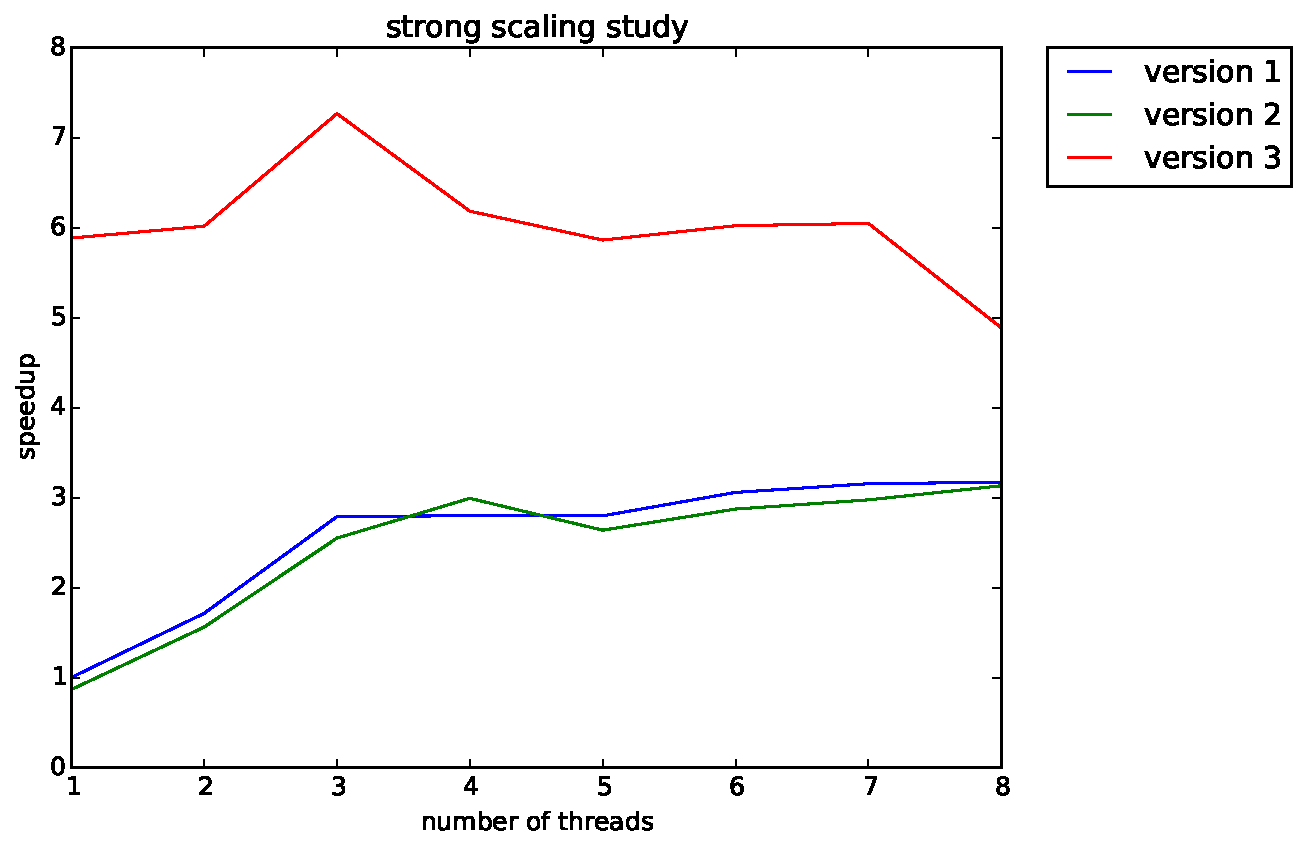
\includegraphics[width=0.85\textwidth] {timing_strong}
        \end{center}
      \label{aload0}
      \caption{strong scaling}
  \end{subfigure}
  \begin{subfigure}
      \centering
        \begin{center}
      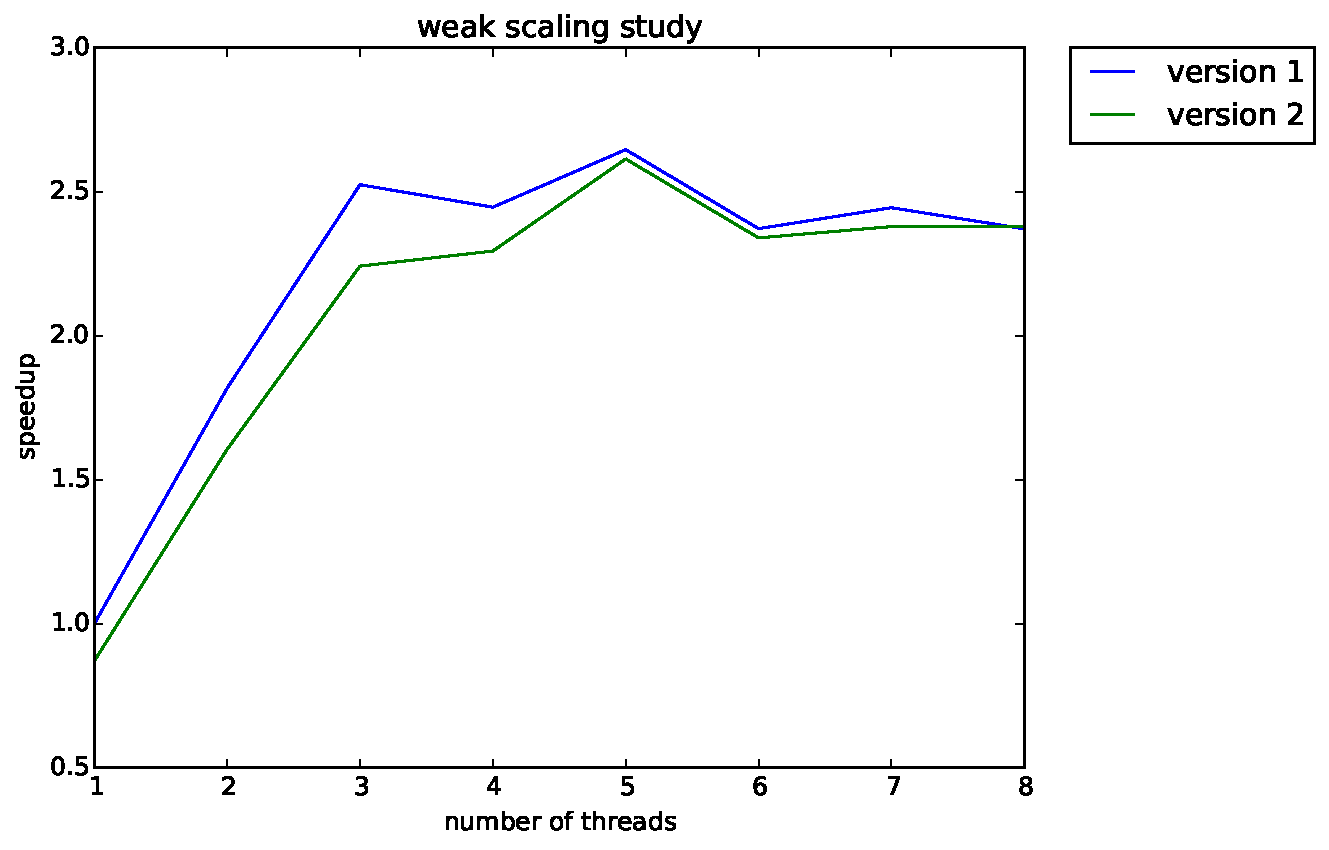
\includegraphics[width=0.85\textwidth] {timing_weak}
        \end{center}
      \label{aload1}
      \caption{weak scaling}
  \end{subfigure}

\end{figure}






\section*{Reference}

(1) D. Bindel, Shallow water simulation, Applications of Parallel Computers (CS 5220), Fall 2015.
\\
(2) D. Bindel, Optimization and analysis tools, Applications of Parallel Computers (CS 5220), Fall\\ 2015.
\\
(3) D. Bindel, Shallow Water Simulation, https://github.com/dbindel/water, 2015.
\\
(4) B. Barney, OpenMP, https://computing.llnl.gov/tutorials/openMP.
\\
(5) G. Jiang and E. Tadmor, Nonoscillatory Central Schemes For Multidimensional Hyperbolic\\ Conservation Laws, {\em SIAM Journal on Scientific Computing}, 19(6), 1892$-$1917.

\end{document}





